\chapter{Preliminary Analysis}\label{chapter:PA}


\section*{Introduction}
\addcontentsline{toc}{section}{Introduction}
Following that, having reviewed the theoretical concepts that will help to improve the understanding of the project, we proceed to the requirements analysis and technical specifications stage. In this second chapter, we construct the functional study of the project and minor sequence diagrams of use case and technical study of the technologies used in the project.

\section{Functional study}
The functional study is a crucial step in the process of understanding the subject and the activities that will be performed. It normally features the actors, the functional responsibilities of these actors and the dynamic between the different actors in the form of UML diagrams.

\subsection{Identifying the system actor}


The key actor in Uni-world is the \textbf{Student}, who will benefit from the application's functionalities. \\
The application will only permit students to use it by providing additional authentication details such as submitting a university e-mail address, the form of which is well specified.

\subsection{Identifying functional requirements}
\textbf{Functional requirements represent the features provided by the system to meet the user's expectations, listing the key functionalities that uni-world offers:}\\
The application comprises the following modules : 
\begin{itemize}
    \item User Management Module:\\
The User Management Module covers the application of the actual management of the users. An example of it is password login, user registration, activation of an account, password reset, and other details about the account. This module provides users with as much simplicity and security as possible while signing up or logging in to the service.
\begin{itemize}
\item Login: \\
Confirm the validity of the student by entering the university and password that is set by the student.
\item Registration: \\
Easy registration form with input values including name, e-mail address ,password and other data that are useful to build the user profile.
E-mail address verification is used to confirm the existence of an account and prevent spam. It can also be used to determine the authenticity of the user and his or her university.
\item Account Activation:\\
As for the link activation of new users, the emails will be sent.
Short accountability of account activation related to increased brand recognition.
\item Password Reset:\\
Password change mechanism over email using a trusted link.
User confirmation or the extra dilemma in changing the password to enhance security features.
\item Account Management:\\
Menu entries can be used to input new personal details of the user, to change passwords, and to set the level of privacy.
\end{itemize}    
    \item Profile Swiping Module:\\
This specific learning module is to encourage students to make friends and interact with each other through a feature of swiping cards like the Bumble application. This is useful to help a student, for example, if they want to meet new people or if they do not want to interact with people, this feature allows it.
\begin{itemize}
\item Profile Creation: \\
We can keep identity information by making personal and unique profiles with profile pictures, about oneself details, and more.
\item Swiping Mechanism: \\
Like the real world, the app or site allows you to ‘swipe right’ to indicate you are interested and ‘swipe left’ to show the opposite.
Inclusion of algorithms through which the application can identify the list of profiles with, which the user is likely to share a common interest and/or mutual friends.
\item Matching: \\
Students tap on each other’s picture to match once two students have swiped right, they are matched.
An alert message is sent to the two users regarding the match.
\item Chat Initiation: \\
Matched users have the privilege of chatting each other somewhere within the App.
End-to-end also means having a secure and private chat environment.
\end{itemize}
\item Carpooling Module: \\
Finding ways how to get to school without hiring personal transport is a key concern amongst students, this module caters to that aspect as students will find means to share transport costs.\\
\begin{itemize}
\item Creating Carpool Offers: \\
Carpool offers can be offered and posted by the users; with additional information such as the destination, time, and number of seats available among others.
\item Browsing Carpool Offers: \\
This way the students can see all the Carpool offers present in their vicinity.
There are various fields to filter its searches so that their offers will meet their desired time schedule and preferred location.
\item Expressing Interest: \\
It means showing interest in carpool offer by swiping right hand side.
If a user does not want to claim an offer, he can just swipe left on the page.
\item Offer Acceptance: \\
Interests of users are promptly alerted to the offer owners.
Owners are also able to view all the interest requests that are made to them, and they have the privilege of either approving or rejecting them.
An alert message is sent to the two users regarding the match.
\item Chat for Carpool Coordination: \\
After an acceptance, there starts a chat between the owner of the carpool offer and the intended user.
Is useful in co-coordinating and sealing all the details of a carpool and other related matters.
\end{itemize}
    \item Notifications Module: \\
The Notifications Module makes sure that the user will always be notified on activities and updates that are taking place within the application.
    \begin{itemize}
    \item Real-time Notifications: \\
Notifications of new messages, date arrivals, people interested in carpooling etc.
\item Customizable Notification Settings: \\
They are able to do this under the application settings tab where they have the ability to turn off notifications from the application.
    \end{itemize}
\end{itemize}

\subsection{Identifying non-functional requirements}
Nevertheless, non-business requirements are not related to business directly. however, this aspect must be included in the requirements definition to achieve better application quality. Our solution must ensure for our solution to be effective it must meet the following :
\begin{itemize}
    \item Maintainability: or in other words, the level to which an application is known or fixed or enhanced in a way to pose no challenge to the new developers working on the application in terms of code readability and implementation and this is achieved by proper documentation of the code and good comments placed at relevant places in the code and place appropriate names for the class, variables and methods used in the application.
    \item Usability: the application must be easily manipulable and has clean, updated high and fluid interaction and suited for both small screen mobile and larger screen and bigger. This is made possible given that the jetpack compose improves the making of interfaces that are easy to use together with a swipe system.
    \item Extensibility: Thus, the application is more versatile in terms of it possibility to be developed and implemented and containing more features due to its good initial setup resulting from the usage of design patterns and proper extendable architecture.
    \item Security: the application must be secure and access should be provided through the user rights only. JSON web token can also ensure the authenticity of the user hence reducing on invasions that can be conducted by other unlawful users, The passwords and the messages are also encrypted hence ensuring the user confidentiality.
\end{itemize}


\subsection{ Global Use case diagram}
The use case diagram describes the system's behavior from the user's point of view. It divides its functionalities into use cases that express the needs of its users, as shown in Figure 2.1 below.

\begin{figure}[H] 
            \centering
            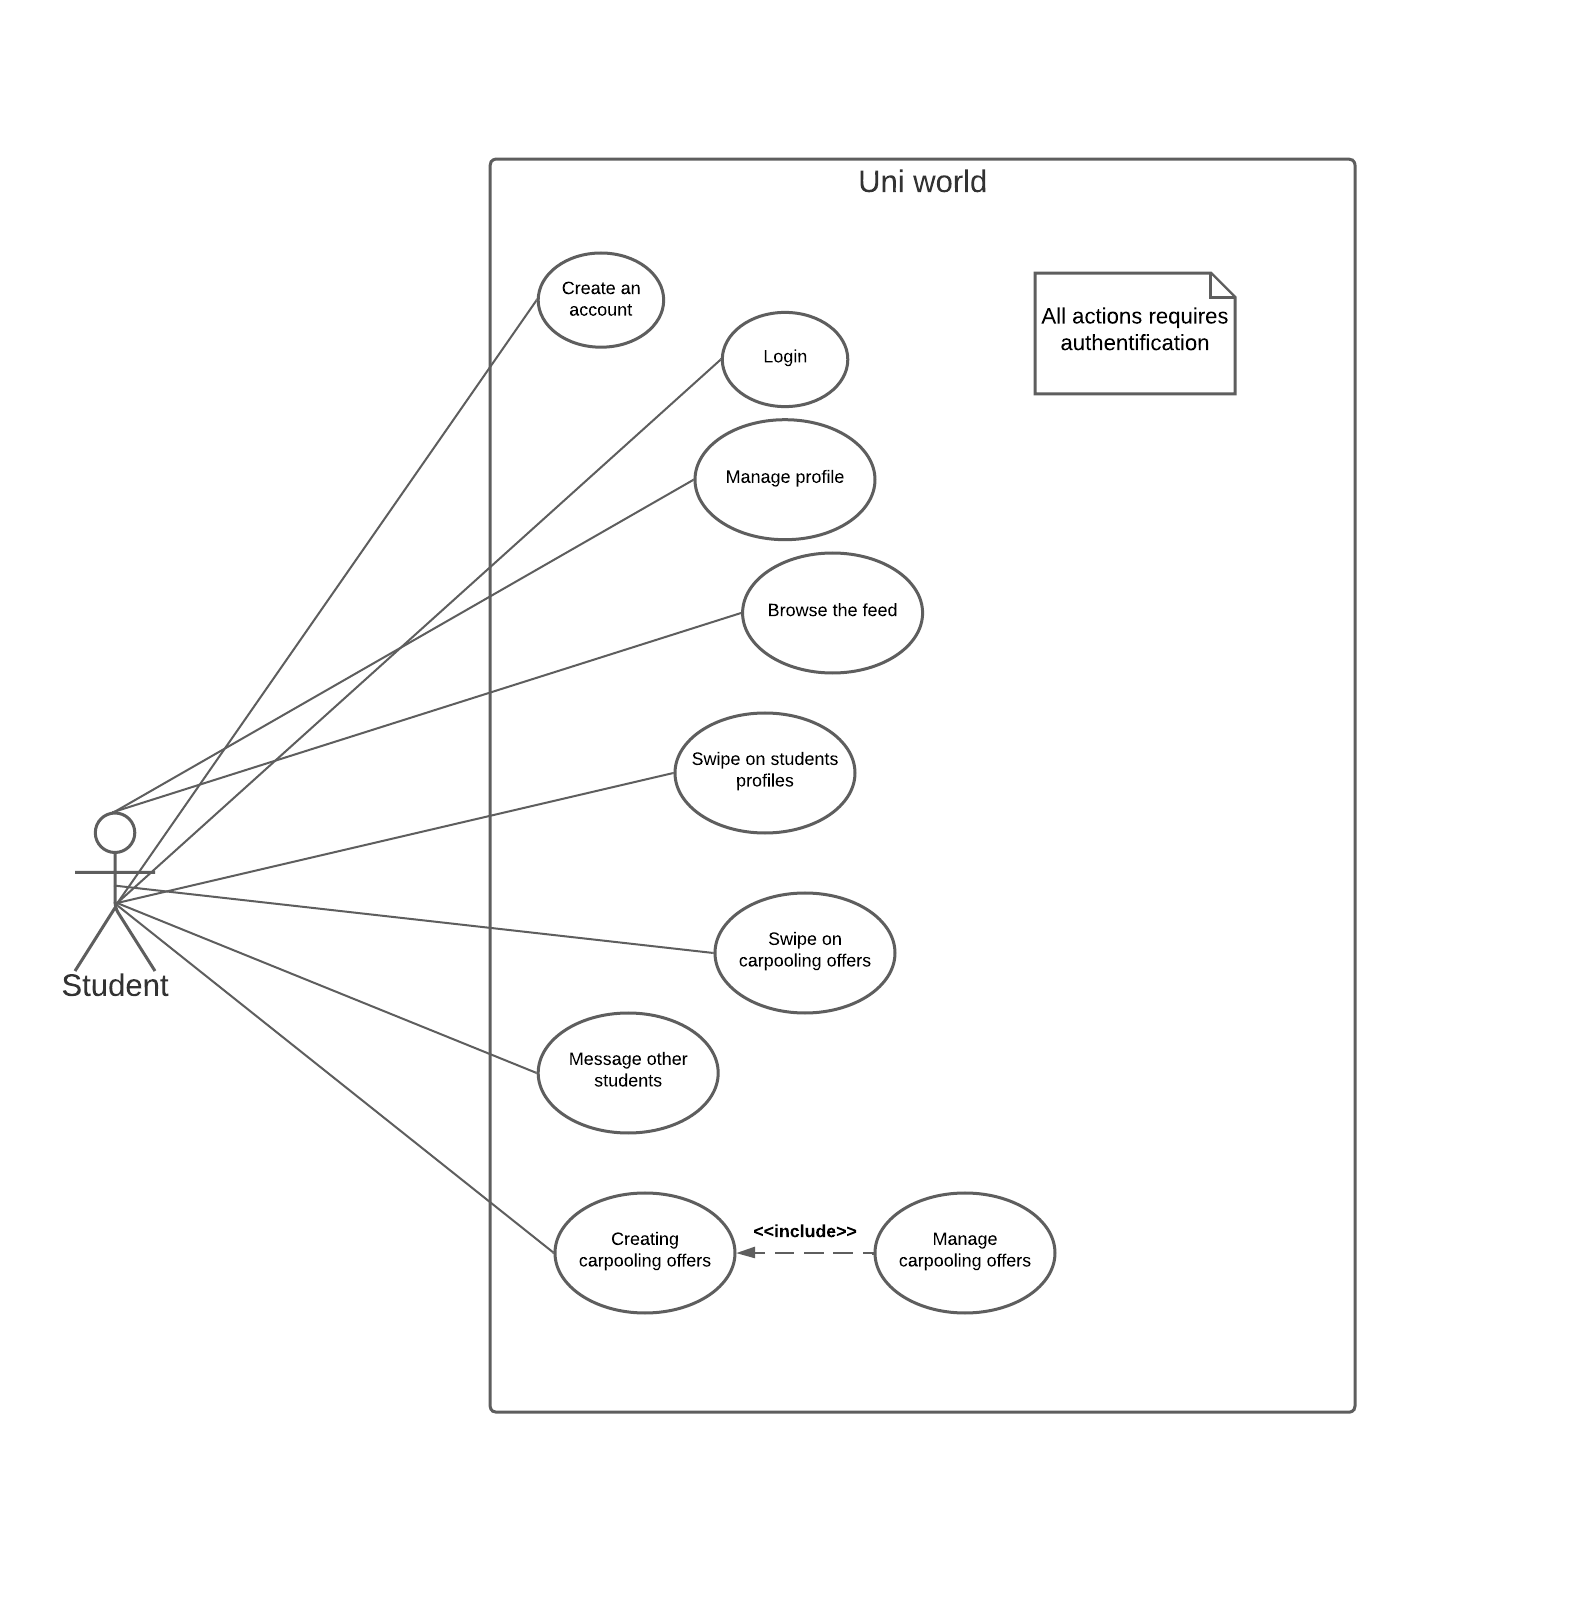
\includegraphics[scale=0.5]{diagrams/global use case.png}
            \caption{Global use case diagram} 
            \label{fig: Global use case diagram}
\end{figure}
\space
\section{Project management using Scrum}
Referring to Chapter 1, page 16, subsection 1.6.3, it is discussed that the Project is managed according to SCRUM methodology because of its efficiency and application to the project.

\subsection{Product backlog}

The Product Backlog is the working document of the project that contains all the anticipated functionalities.
of the product that is used often, these are commonly known as user stories.
that all residues related to the products lies with the priority of the Product Owner
the User Stories of the Product Backlog using the MoSCoW method:the User Stories of the Product Backlog using the MoSCoW method:
\begin{itemize}
    \item M (Must Have) : it stands for what needs to be done. It is important to conclude this criterion to fully meet project objectives. They classified it as high criticality.
    \item S (Should Have) : This is a must adjustment that must be made whenever possible. If not, it can be done later so as to fit the time line of the project.
    \item C (Could Have) : This is a need that is highly desirable but, unlike the essential needs, can be satisfied without having much effect on the rest of the tasks in the day.
    \item W (Won’t have) : It is optional to implement, but would be an interesting nice to have, though not a must
\end{itemize}
The Product backlog for this project is shown in the table below:

\begin{table}[H]
    \centering
    \begin{tabular}{|p{0.5cm}|p{12cm}|p{2cm}|}
        \hline
ID & User Story & Priority \\
\hline
1 & As a student, I want to register easily and securely & M \\
\hline
2 & As a student, I want to log in to a space reserved for students & M \\
\hline
3 & As a student, I want to show my interest by swiping right on someone so that I can contact them if they like me back & M \\
\hline
4 & As a student, I want to ignore someone I don't find interesting & M \\
\hline
5 & As a student, I want to receive an email to activate my account & C \\
\hline
6 & As a student, I want to receive an email to change my password if I have forgotten it & M \\
\hline
7 & As a student, I want to send and receive messages from my matches & M \\
\hline
8 & As a student, I want to see who likes me so I can decide whether or not to like them back & S \\
\hline
9 & As a student, I want to filter my feed according to many criteria & S \\
\hline
10 & As a student, I want to choose the gender I want to interact with & C \\
\hline
11 & As a student, I want to change my password & M \\
\hline
12 & As a student, I want to switch from social mode to carpool search mode & M \\
\hline
13 & As a student, I want to browse available carpooling offers & M \\
\hline
14 & As a student, I want to show my interest if I find an offer interesting, and ignore offers I don't like & M \\
\hline
15 & As a student, I want to create a carpool offer & M \\
\hline
16 & As a student, I want to manage my carpool offers & M \\
\hline
17 & As a student, I want to see who's interested in my offers & M \\
\hline
18 & As a student, I want to accept or reject other users interested in my offers & M \\
\hline
19 & As a student, I want to receive notifications when I get a match or message & S \\
\hline
20 & As a student, I want to manage my account & M \\
\hline
    \end{tabular}
    \caption{Product backlog}
    \label{Tab: Product backlog}
\end{table}
\subsection{Sprint Planning}
The table below shows the breakdown of the project into user stories for each sprint :
\begin{table}[H]
    \centering
    \begin{tabular}{|p{2cm}|p{6cm}|p{4cm}|}
        \hline
Sprint ID & Title & User Stories \\
\hline
1 & User management & 1-2-5-6-11-20 \\
\hline
2 & Social life features (Uni-match) & 3-4-7-8-9-10 \\
\hline
3 & Carpooling features (Uni-car) & 12-13-14-15-16-17-18-19 \\
\hline
    \end{tabular}
    \caption{Sprint Planning}
    \label{Tab: Sprint Planning}
\end{table}
\section{Class diagram}
As will be seen in the following sections, it is useful to prepare a class diagram to understand each component of this application in detail. This diagram shows all classes which include their attributes and methods and also relations between classes. \\
It becomes important to have this form of presentation to easily comprehend the code’s architecture. This allows the developers to see how the varied parts relate to each other and how they are interconnected, especially in the designing and development phase.

\begin{figure}[H] 
            \centering
            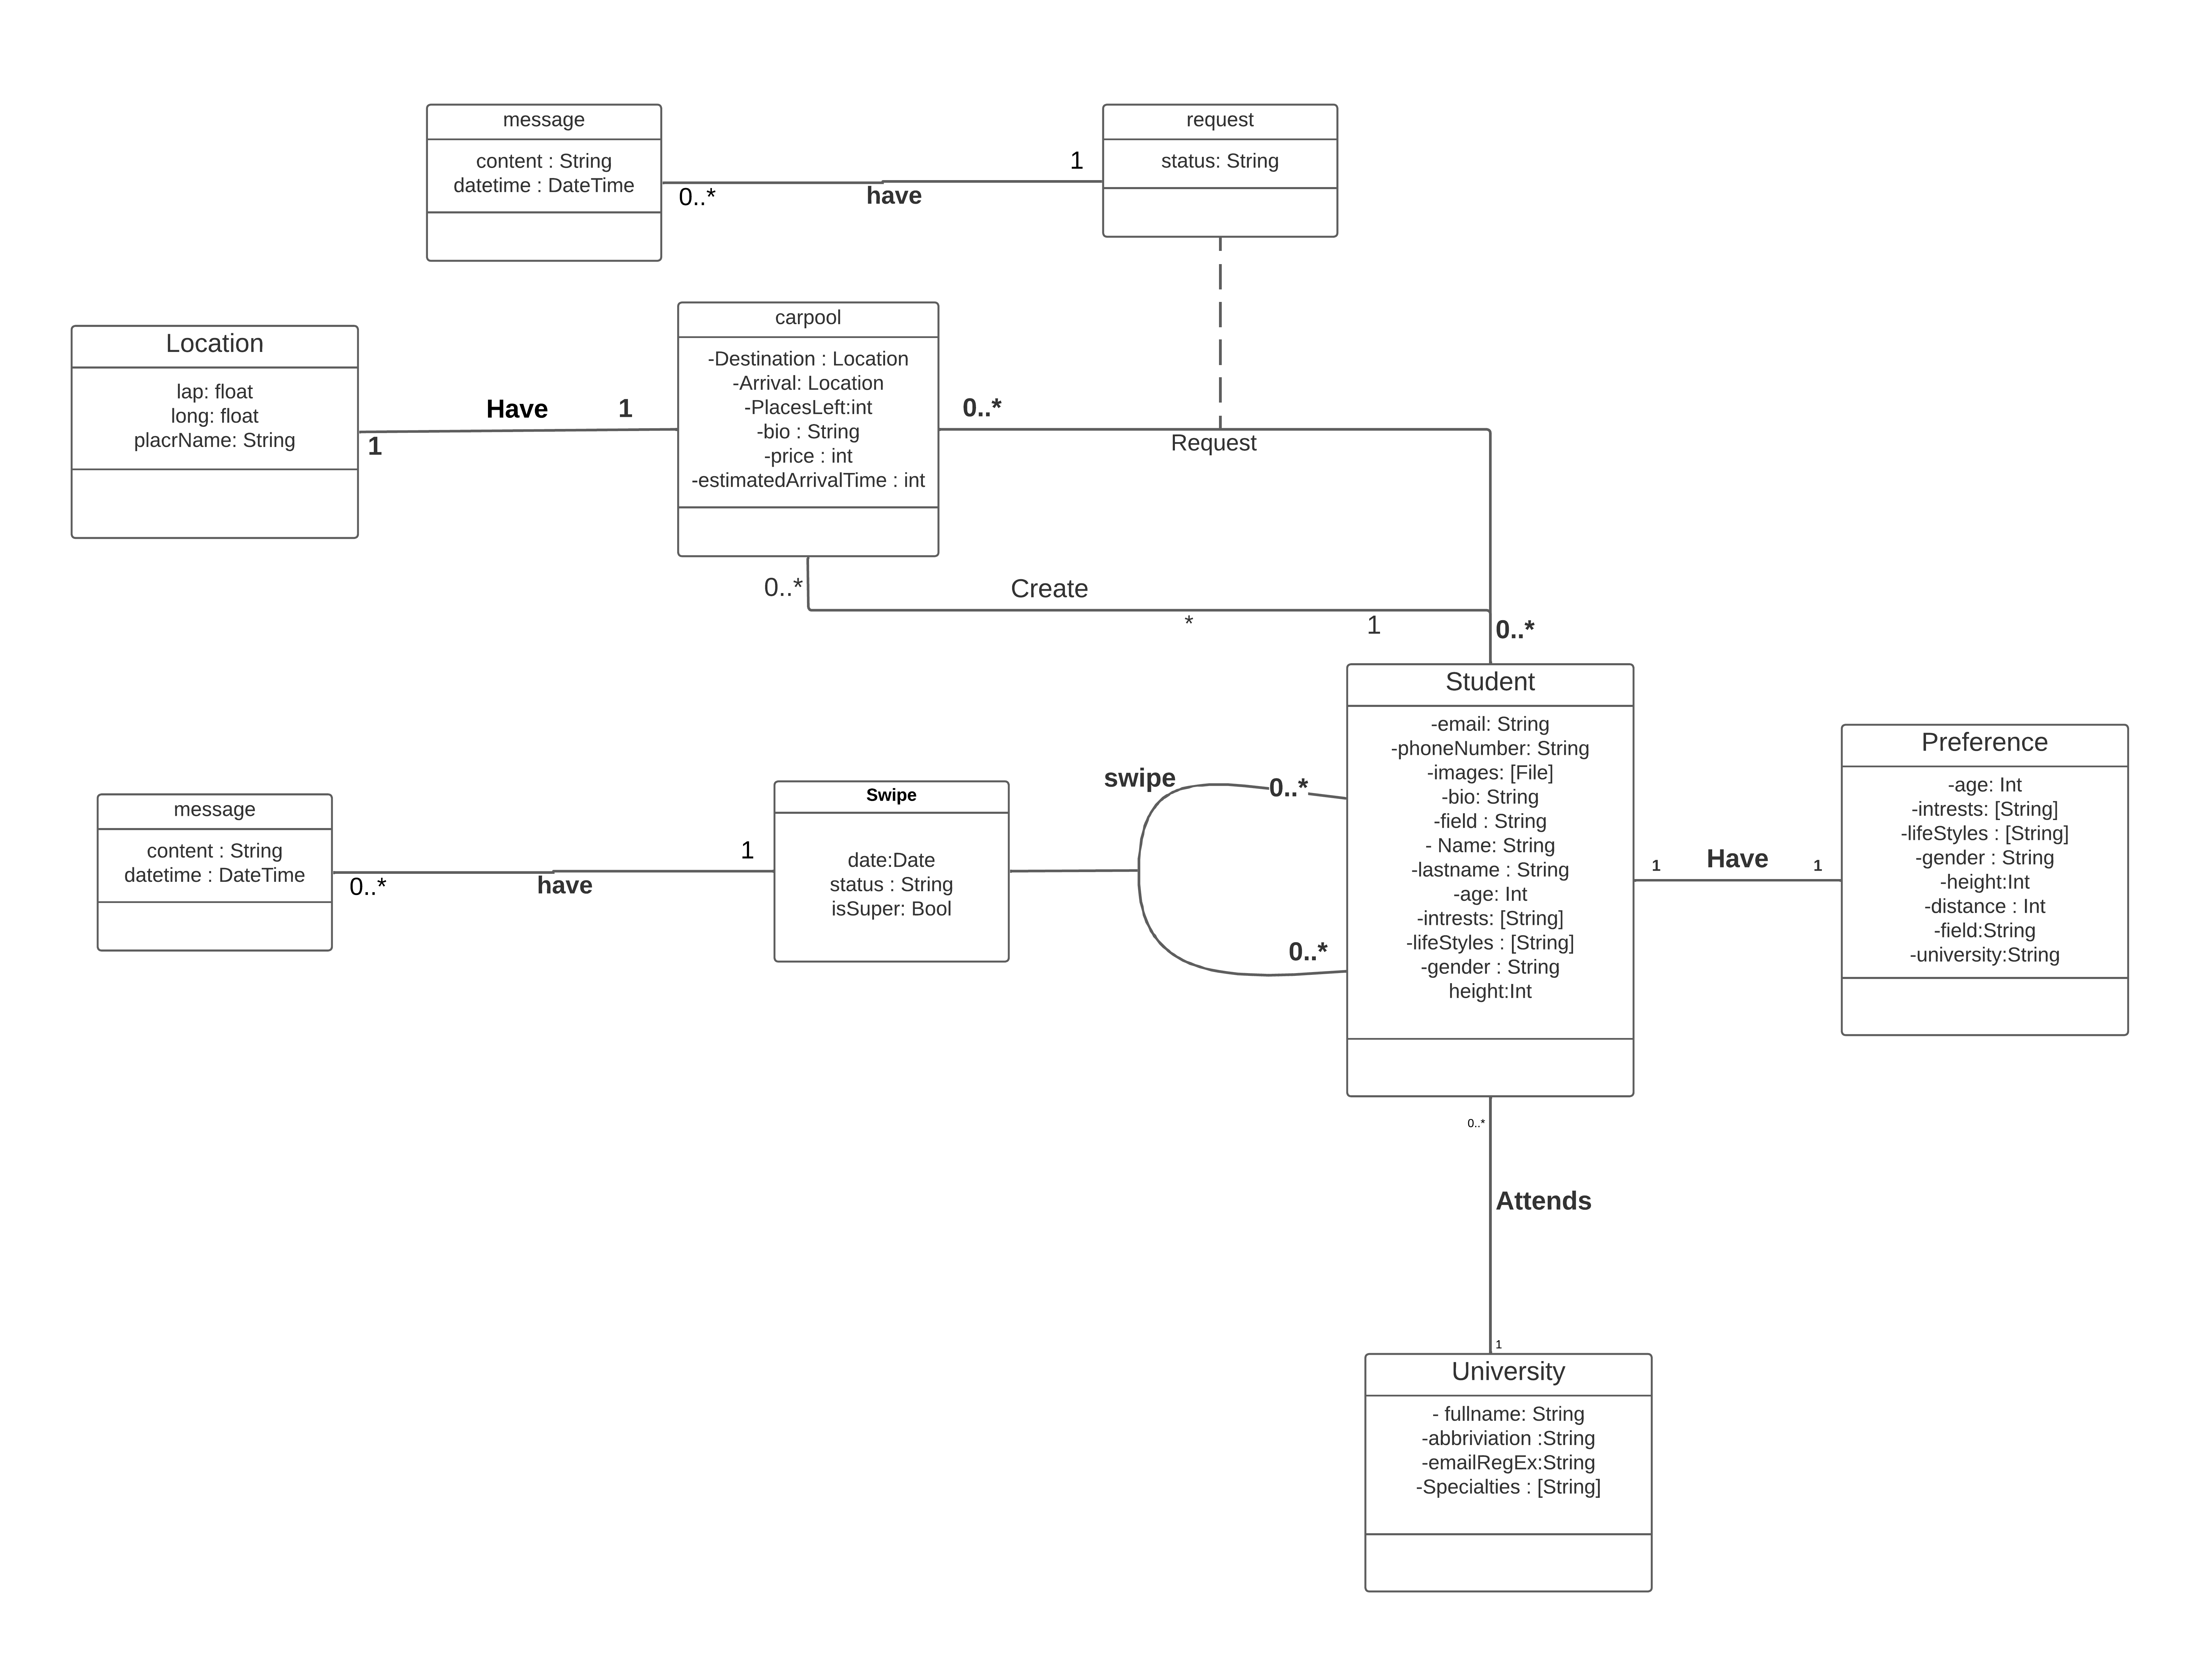
\includegraphics[scale=0.3]{diagrams/class diagram.png}
            \caption{Uni-world's class diagram } 
            \label{fig: Uniworld's class diagram}
\end{figure}

\section{Uni-world architectural conception}
\subsection{Physical architecture}
The physical architecture of our solution requires a hardware infrastructure to guarantee efficient operation of the application. A powerful, reliable server is crucial. For Uni-world, we opted for an N-tier architecture.
Consequently, Uni-world will be structured around three main Tiers, Presentation Tier, Application Tier and the data Tier, each playing a distinct role:
\begin{itemize}
    \item Presentation Tier (Jetpack compose): this layer supports the user interface and experience
    experience on mobile devices. Using the Jetpack compose Framework, it enables you to
    create an intuitive, responsive interface, providing a smooth, seamless user
    experience.
    \item Application Tier (Node .js): this layer is the “brain” of our application, in charge of all business logic and data processing. It is crucial to guarantee the application's performance, security and scalability.
    \item Data Tier (MongoDB): this layer manages and stores the data.
    data. It must guarantee the integrity, consistency and availability of information.
\end{itemize}
\begin{figure}[H] 
            \centering
            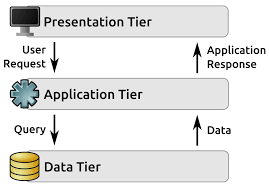
\includegraphics[scale=0.9]{physical archi.png}
            \caption{N-Tier Physical architecture} 
            \label{fig: N-Tier Physical architecture}
\end{figure}
\subsection{Software architecture}
Software architecture refers to the structures that are required for comprehending a software system while also constituting the practice of designing such structures and systems. Every structure is better described as software entities, interconnections between the entities, and attributes of both entities and relations. \\
In this application, we have adopted the CLEAN architecture and MVVM architectural pattern for the presentation section as outlined in the following figure.

\begin{figure}[H] 
            \centering
            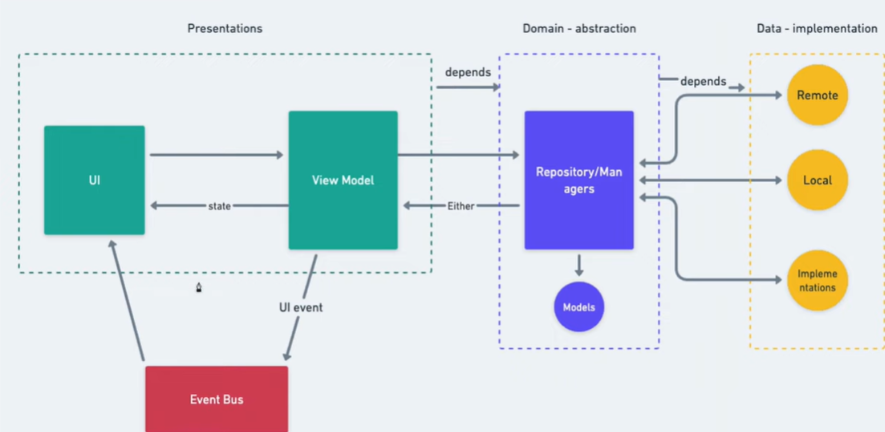
\includegraphics[scale=0.8]{mvm.png}
            \caption{Software architecture : CLEAN architecture and MVVM } 
            \label{fig: CLEAN architecture and MVVM}
\end{figure}

\section{Hardware resources}
The table 2.3 shows the hardware setup used in our project.
\begin{table}[H]
    \centering
    \begin{tabular}{|p{4cm}|p{6cm}|}
        \hline
        Owner & Bairem khedhri\\
        \hline
        RAM & 16,0 GB \\
        \hline
        CPU & 11th Gen Intel(R) Core(TM) i5-11400H @ 2.70GHz   2.69 GHz \\
        \hline
        Storage & 512 Go SSD \\
        \hline
        Operating system  & Windows 11 Professional 64-bit \\
        \hline
    \end{tabular}
    \caption{Hardware resources}
    \label{Tab: Hardware resources}
\end{table}

\section{Work environment}
For a project as heavy as uni-world, I need several tools and software to help me improve the project, such as : \\
\begin{itemize}
    \item \textbf{Figma:} A tool used in the development of the application, particularly in the UX/UI 
    design where the application is designed and a prototype made.
        \begin{figure}[H] 
            \centering
            
\includegraphics[scale=0.03]{logos/Figma-logo.png}
            \caption{Figma logo } 
            \label{fig: Figma logo}
        \end{figure}
    \item \textbf{Github:} is a software development platform which enables developers to 
    build, host and collaborate on code. This one integrates git software, which adds distributed 
    version control of Git plus, access control, bug tracking, Software requests features, task management, continuous integration, and wikis for every project.
        \begin{figure}[H] 
            \centering
            
\includegraphics[scale=0.15]{logos/github-logo.png}
            \caption{Github logo } 
            \label{fig: Github logo}
        \end{figure}
    \item \textbf{Lucidchart:} A fully managed cloud based tool to create diagrams, data visualization and concept maps. It also offers users powerful features for modeling sophisticated information in a very easy and graphical manner.
        \begin{figure}[H] 
            \centering
            
\includegraphics[scale=0.2]{logos/lucichart-logo.png}
            \caption{Lucidchart logo } 
            \label{fig: Lucidchart logo}
        \end{figure}
    \item \textbf{Android Studio:} Is the integrated development environment or IDE is specifically for developing android applications. It provides a full and optimised environment for the development of applications for the Android system.
            \begin{figure}[H] 
                \centering
                
\includegraphics[scale=0.2]{logos/android-studio-logo.png}
                \caption{Android Studio logo } 
                \label{fig: Android Studio logo}
            \end{figure}    
    \item \textbf{Visual studio Code:} is this cross-platform code editor developed by Microsoft for MacOS, Windows and Linux operating systems, 
    it support native for many popular programming languages.
            \begin{figure}[H] 
                \centering
                
\includegraphics[scale=0.07]{logos/visual-studio-code-logo.png}
                \caption{Visual studio Code logo } 
                \label{fig: Visual studio Code logo}
            \end{figure} 
    \item \textbf{Postman:} This tool is one of the preferred to deal with RESTful API. It is a tool that enables and simplifies the launching, evaluating and the quick use of http requests for efficiency.
        \begin{figure}[H] 
            \centering
            
\includegraphics[scale=0.2]{logos/postman-logo.png}
            \caption{Postman logo} 
            \label{fig: Postman logo}
        \end{figure}
\end{itemize}
\section{Languages and Frameworks}
\begin{itemize}
    \item \textbf{Kotlin:} Is a statically typed, high-level programming language that can be used practically anywhere. Mostly know for its Android development and API creation.
        \begin{figure}[H] 
            \centering
            
\includegraphics[scale=0.04]{logos/kotlin-logo.png}
            \caption{Kotlin logo } 
            \label{fig: Kotlin logo}
        \end{figure}
    \item \textbf{Jetpack Compose:} Is a modern UI toolkit for Android that makes apps more intuitive with less code, easier maintainability and better runtime performance. It makes it easy to build an one-layer of view in your app with less code,compitable and intergrated well into other Jetpack libraries,makes all short work dynamic UI updates according to data changes.
        \begin{figure}[H] 
            \centering
            
\includegraphics[scale=0.06]{logos/jetpack-compose-logo.png}
            \caption{Jetpack Compose logo } 
            \label{fig: Jetpack Compose logo}
        \end{figure}
    \item \textbf{Javascript:} Is an object oriented-structured and a high level programming language which finds its applicability mainly in the creation of Web pages. It allows the dynamic content of the websites, forms validations, and control of multimedia objects. Born initially as a 
    client-side scripting language, JavaScript has evolved to be an essential technology in web development that operates both on the client and server-side for the development of interactive applications based on html and CSS.
        \begin{figure}[H] 
            \centering
            
\includegraphics[scale=0.2]{logos/javascript-logo.png}
            \caption{Javascript logo } 
            \label{fig: Javascript logo}
        \end{figure}
    \item \textbf{Node JS:} Is a runtime environment, it provides the environment of executing JavaScript on server side. Being constructed on Chrome’s V8 JavaScript engine, it is beneficial for creating applications with high efficiency and scalability. 
    Node. js is superb in dealing with the asynchronous events and real time data; this makes it a perfect choice in Web applications, APIs, and micro services.
            \begin{figure}[H] 
                \centering
                
\includegraphics[scale=0.5]{logos/node-logo.png}
                \caption{Node JS logo } 
                \label{fig: Node JS logo}
            \end{figure}    
    \item \textbf{MongoDB:} Is a NoSQL DBMS and is regarded as flexible and highly scalable. Data is stored in JSON-like documents and it offers therefore excellent flexibility regarding changing structures of the saved data. MongoDB is perfect for today’s applications because it provides superior querying and indexing functionality alongside the capacity to manage massive amounts of unstructured or semi-structured data.
            \begin{figure}[H] 
                \centering
                
\includegraphics[scale=0.3]{logos/mongo-logo.png}
                \caption{MongoDB logo } 
                \label{fig: MongoDB logo}
            \end{figure} 
        \end{figure}
\end{itemize}

\section*{Conclusion}
After the requirements specification analysis, the conceptual study and the new hardware and software environment for “uni-world”, we are in Sprints development for the progressive incarnation of our project in Sprints.